\documentclass[a4paper]{scrartcl}

%\usepackage{showframe}
\usepackage[margin=2cm,footskip=.7cm]{geometry}
\usepackage{enumitem}
% \usepackage{fourier}
\usepackage{xcolor}
% \usepackage{abkuerzungen}
\usepackage{hyperref}
\usepackage{amsmath}
\usepackage{../../ISASmacros/isasmathmacros}

\usepackage{pdfpages}


\newcommand{\sA}{\ensuremath{\mathsf{A}}}
\newcommand{\sAB}{\ensuremath{\mathsf{AB}}}
\newcommand{\sB}{\ensuremath{\mathsf{B}}}
\newcommand{\sBA}{\ensuremath{\mathsf{BA}}}
\newcommand{\sC}{\ensuremath{\mathsf{C}}}

\newcommand{\cest}{\ensuremath{\cvec{\gamma}}}
\newcommand{\cerest}{\ensuremath{\ervec{\gamma}}}
\newcommand{\cmat}{\ensuremath{\mat{\Gamma}}}
\newcommand{\tmat}{\ensuremath{\widetilde{\mat{\Gamma}}}}

\newcommand{\gainA}{\ensuremath{\mat{K}}}
\newcommand{\gainB}{\ensuremath{\mat{L}}}

% \newcommand{\fus}{\ensuremath{\op{fus}}}

% \newcommand{\CI}{\op{CI}\xspace}
% \newcommand{\EI}{\op{EI}\xspace}
% \newcommand{\ICI}{\op{ICI}\xspace}
% \newcommand{\BC}{\op{B\!/\!C}\xspace}
% \newcommand{\ind}{\op{s}\xspace}
\newcommand{\ind}{\op{in}\xspace}
\newcommand{\opt}{\cmat}


\newcommand{\excmat}{\ensuremath{\mat{\Gamma}'}}
\newcommand{\excest}{\ensuremath{\cest'}}
% \newcommand{\exoptmat}{\ensuremath{\mat{C}_{\excmat}}}
\newcommand{\exoptmat}{\ensuremath{\mat{C}'_\EI}}

%\RequirePackage[mathscr]{euscript}
%\RequirePackage{bbding}
%\RequirePackage{scalefnt}
%\RequirePackage{mathtools}
% This was enabled but makes the text look ugly
%\RequirePackage[T1]{fontenc}


%%% COLOR DEFINITIONS

% KIT Colors
\definecolor{kitgreenex}{RGB}{0,152,131}
\definecolor{kitblueex}{RGB}{52,115,186}
\definecolor{kitmaygreen}{RGB}{119,184,38}
\definecolor{kityellow}{RGB}{255,228,0}
\definecolor{kitorange}{RGB}{247,154,0}
\definecolor{kitbrown}{RGB}{182,130,28}
\definecolor{kitred}{RGB}{187,25,23}
\definecolor{kitpurple}{RGB}{190,0,126}
\definecolor{kitcyanblue}{RGB}{0,167,227}
% Own Definitions
\definecolor{grey}{RGB}{150,150,150}


\definecolor{nblue}{RGB}{54,95,145}

%%% FONTS
%\setkomafont{pageheadfoot}{\small\color{darkgray}}
%\setkomafont{pagefoot}{\normalfont\color{darkgray}}
%\setkomafont{pagenumber}{\color{darkgray}}
%\setkomafont{captionlabel}{\small\bfseries\color{darkgray}}
\setkomafont{disposition}{\bfseries}
\setkomafont{section}{\normalfont\large\bfseries}
\setkomafont{subsection}{\normalfont\bfseries}
\setkomafont{author}{\normalfont}
\setkomafont{date}{\normalfont}


%%% PARAGRAPH LAYOUT
\setlength{\parindent}{0mm}
\setlength{\parskip}{6pt}


%%% REBUTTAL COMMANDS
\newenvironment{rebuttal}{\begin{enumerate}[label={\color{grey}\thesection.\arabic{enumi}},leftmargin=0pt,ref=\thesection.\arabic{enumi}]}{\end{enumerate}}
\newcommand{\reviewtext}[1]{{\color{nblue} #1}}
\newcommand{\papertext}[1]{\emph{``#1''}}

%%% HYPERREF SETUP
\hypersetup{
        colorlinks = true,
        linkcolor = kitgreenex
}

%%%%%%%%%%%%%%%%%%%%%%%%%%%%%%%%%%%%%%%%%%%%%%%%%%%%%%%%%%%%%%%%%%%%%%%%

\title{\boldmath Distributed Range-Only Localisation that Preserves Sensor and Navigator Privacies}
\subtitle{Response to Reviewers' Comments - Submission IEEE-TAC 21-1548}
\author{Marko Ristic\and Benjamin Noack\and Uwe D. Hanebeck}

%       .d8888b.  888                     888
%      d88P  Y88b 888                     888
%      Y88b.      888                     888
%       "Y888b.   888888  8888b.  888d888 888888
%          "Y88b. 888        "88b 888P"   888
%            "888 888    .d888888 888     888
%      Y88b  d88P Y88b.  888  888 888     Y88b.
%       "Y8888P"   "Y888 "Y888888 888      "Y888

\begin{document}

\maketitle

Dear Dr. Zhiwei Gao,\\
Dear Reviewers,

Thank you all for your detailed reviews and for finding the manuscript suitable for publication. In this letter, we will address the remaining editor and reviewer comments and describe any changes made to the manuscript. Throughout this response, reviewers' comments are in \reviewtext{blue}. 

Sincerely,\\
Marko Ristic, Benjamin Noack, and Uwe D. Hanebeck

%      8888888888     888 d8b 888
%      888            888 Y8P 888
%      888            888     888
%      8888888    .d88888 888 888888 .d88b.  888d888
%      888       d88" 888 888 888   d88""88b 888P"
%      888       888  888 888 888   888  888 888
%      888       Y88b 888 888 Y88b. Y88..88P 888
%      8888888888 "Y88888 888  "Y888 "Y88P"  888



\section*{Response to the Editor's Report}
\def\thesection{E}
\begin{rebuttal} %\setcounter{enumi}{-1}
\item \reviewtext{I am pleased to inform you that the paper is acceptable for publication in the Transactions provided that you can make the modifications described below. The reviewers would like the authors to clarify some concerns such as the assumption of the EKF design, private sensor variance information, and research motivation and challenge, and so forth.}

We are glad to hear the paper is acceptable for publication and have responded to each of the reviewer comments below, hoping to clarify all remaining concerns.

\end{rebuttal}

%      8888888b.                         d888
%      888   Y88b                       d8888
%      888    888                         888
%      888   d88P .d88b.  888  888        888
%      8888888P" d8P  Y8b 888  888        888
%      888 T88b  88888888 Y88  88P        888
%      888  T88b Y8b.      Y8bd8P         888
%      888   T88b "Y8888    Y88P        8888888



\section*{Response to the Comments of Reviewer 1 (242571)}
\def\thesection{R1}
\begin{rebuttal}
\item \reviewtext{Thank you for updating the manuscript and most of the concerns have been addressed well in the response letter.}

We are happy to hear this is the case, thank you.

\item \reviewtext{However, there is one problem still confused me. The authors claimed that the Gaussian assumption has been removed in the revised version, however, the EKF (EIF) was still used for prediction (Eqs. 26-27). Basically, the EKF is based on the Gaussian assumption and the prediction is obtained in the sense of mean value. Then, the non-Gaussian dynamics would affect the prediction performance using EKF if the Gaussian assumption is removed. My point is 1) if the assumption is removed, please explain the non-Gaussian influence from the EKF or 2) if the Gaussian assumption remains in the manuscript, please explain from the noise comes from in physics sense.}

We regret that there was some confusion about the prediction step of the presented localisation algorithm. Equations $26$-$27$ are the EKF (EIF) update equations (rather than the prediction equations), resulting in updated terms $\vec{y}_{k|k}$ and $\mat{Y}_{k|k}$ from the predictions $\vec{y}_{k|k-1}$ and $\mat{Y}_{k|k-1}$. The Gaussian assumption has indeed been removed from the system model, and obtaining the predictions $\vec{y}_{k|k-1}$ and $\mat{Y}_{k|k-1}$ can be computed using any local filter (linearising or otherwise) as mentioned in Section V. The Gaussian assumption that remains is only present in the measurement model, as is a commonly done to simplify the modelling of sensors, and the non-linear distance-measurement function $h_i$ is linearlised by an appropriate EKF filter for the localisation update step only. We hope this clarifies equations $26$-$27$ and the use of the EKF.

\end{rebuttal}

%      8888888b.                         .d8888b.
%      888   Y88b                       d88P  Y88b
%      888    888                              888
%      888   d88P .d88b.  888  888           .d88P
%      8888888P" d8P  Y8b 888  888       .od888P"
%      888 T88b  88888888 Y88  88P      d88P"
%      888  T88b Y8b.      Y8bd8P       888"
%      888   T88b "Y8888    Y88P        888888888



\section*{Response to the Comments of Reviewer 2 (242573)}
\def\thesection{R2}
\begin{rebuttal}
\item \reviewtext{The authors have significantly improved the readability of the paper. The contribution is significant enough for privacy preserving state estimation.}

We thank you for the comment and are glad that the contribution is found significant.

\item \reviewtext{However, this reviewer still have few comments:

1- It could be interesting to comment why sensor variance is a private information. Why is it crucial to preserve it if measurements are already protected?}

This is a good question that had not been elaborated in the work. The key reason that any sensor-specific information (such as its measurement noise variance) is considered private is that it may hold identifying data if analysed by an adversary. For example, a particular model of sensor may be identified from its measurement noise variance, enabling a targeted attack (cyber or physical) against that sensor. We have made a change to the introduction section to clarify this reasoning.

\item \reviewtext{2- In the sentence 'homomorphic encryption is used to make time-independent model-free location estimates where an estimator does not learn sensor measurements or locations.; Shouldn't be 'cannot learn'?}

Thank you for pointing this out, we have added the change to the manuscript.

\item \reviewtext{3- In problem statement 'we consider the context of privacy-preserving range sensor navigation, where we want no sensor to learn information about the navigator or other sensors beyond their local measurements, and the navigator to learn no information about individual sensors beyond its location estimate.', please specify type of information.}

We regret that this was not clear to the reviewer. We refer to leakable content as arbitrary information to stress that \textit{nothing} can be leart. That is, neither the information we can predict the importance of (such as state estimates or sensor locations), nor that for which we cannot. This is common in cryptography, as no assumptions on the methods or intentions of adversaries can be made. We have updated the sentence to try and make this clearer and note that examples of information that should not be learnt (state estimates and sensor locations) have been given in the preceeding section.

\item \reviewtext{4- Indistinguishable weights: what would happen if the sensor learns navigator weights?}

This relates to the abstraction from the previous response. Since a meaningful cryptographic definition cannot make assumptions about what leakable information might be useful, we cannot state what would happen. As the weights originate from the navigator and we do not want sensors to learn any information from the navigator, we can say that no new information should be leart from the weights (and therefore require cryptographic indistinguishabilty of weights). In the concrete scheme presented later, it can be seen that the weights correspond to elements of the navigator's state estimate vector, which is stated as an example of information that must remain private to the navigator. We hope this makes the meaning and reasoning of indistinguishability clearer.

\item \reviewtext{5- Fix the following sentence: 'If an attacker compromises the navigator, they have control over the weights,'}

Unfortunately, we are unable to find an issue with the stated sentence and have asked additional native English speakers that have also agreed that the sentence looks correct. In case the use of ``they'' (rather than ``he'' or ``she'') is being referred to, it is the formal grammatical pronoun for a person when gender is not specified.

\item \reviewtext{6- Define IND-CPA.}

We are sorry for the confusion, the first use of the term ``Indistinguishability under the Chosen Plaintext Attack (IND-CPA)'' is in section II.A and has been referenced (reference [21]). The full cryptographic game which defines it was present in the appendix of the initial submission but removed due to initial reviews requesting fewer cryptographic background information. We hope this clears up why the definition is only referenced.

\item \reviewtext{7- Simulation: The authors have found that 1.7 s are needed for each
computation step, is that compatible with real-time operation?}

My response.

\item \reviewtext{8- Can you comment why quantization noise, involved in the encryption-decryption schemes, isn't taken into account in the filter equations?}

We're sorry this wan't clearer. 


\dots quantisation noise is negligible when the quantised integer bit size is larger than the bit size of used floating-point numbers


\end{rebuttal}

%      8888888b.                         .d8888b.
%      888   Y88b                       d88P  Y88b
%      888    888                            .d88P
%      888   d88P .d88b.  888  888          8888"
%      8888888P" d8P  Y8b 888  888           "Y8b.
%      888 T88b  88888888 Y88  88P      888    888
%      888  T88b Y8b.      Y8bd8P       Y88b  d88P
%      888   T88b "Y8888    Y88P         "Y8888P"



\section*{Response to the Comments of Reviewer 3 (246951)}
\def\thesection{R3}
\begin{rebuttal}
\item \reviewtext{Comments:

This paper proposes a novel distributed localisation method in the presence of range-only sensors, which preserves both navigator and sensor privacies. The major contribution of this paper is that a novel private linear combination aggregation scheme is proposed, and based on that, a modified extended Kalman filter is also derived. Some comments are given as follows:

1.In this paper, the full names of some abbreviations are not given. For example, in Section I, page 1, left column, “AES”and “RSA”, and in Section I, page 1, right column, “pWSAc” and “pWSAh”.}

My response.

\item \reviewtext{2.The authors should elaborate the advantages and disadvantages of the existing typical cryptographic secrecy scheme and the motivation for proposing private linear combination aggregation scheme in this paper.}

My response.

\item \reviewtext{3.Some symbols are reused. For example, In Section I, Notation, “timestep k” and “will denote encryption and decryption with key k”.}

My response.

\item \reviewtext{4.The authors need to present theoretical computational complexity of the proposed method.}

My response.

\item \reviewtext{5.The authors should state how to measure the performance of the private linear combination aggregation scheme proposed in this paper.}

My response.

\item \reviewtext{6.In practical engineering application, how to balance the relationship between key sizes and computation.}

My response.

\end{rebuttal}

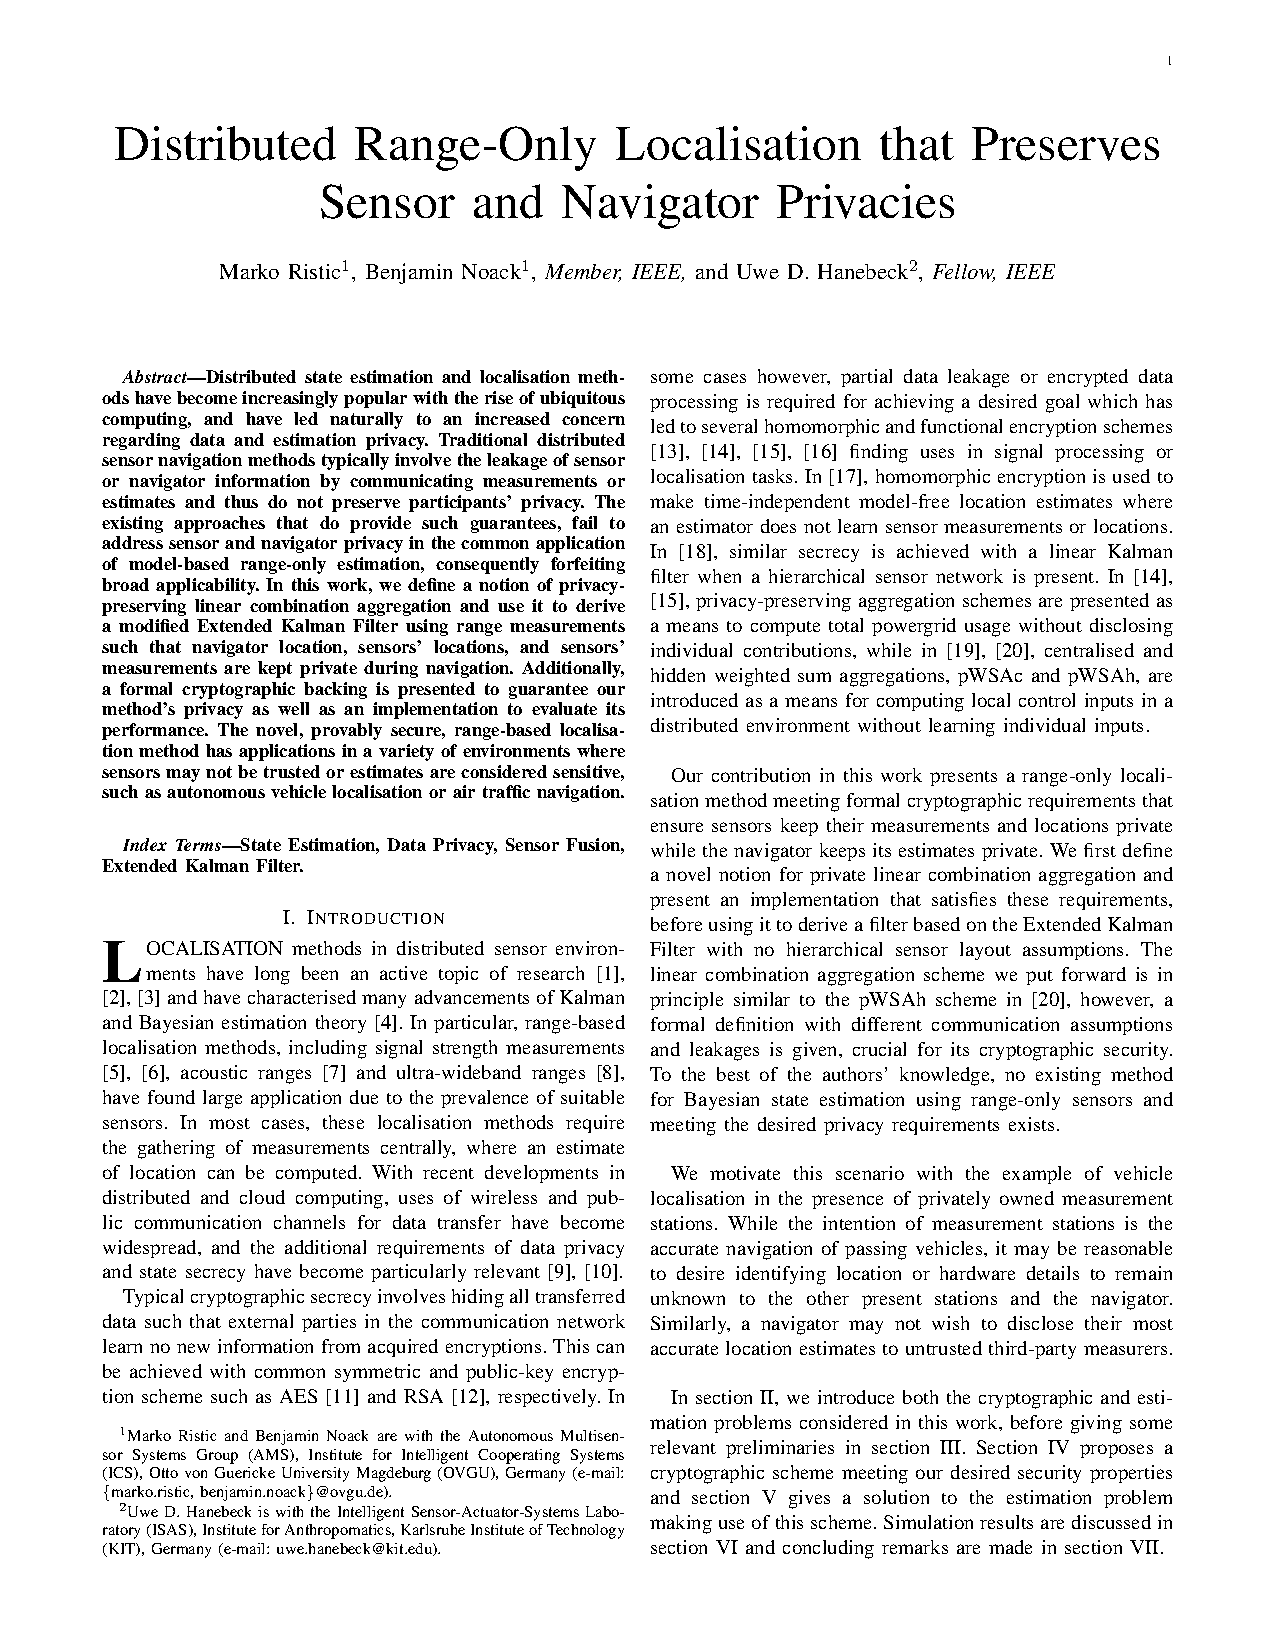
\includepdf[pages=-]{../../diff.pdf}

\end{document}